\documentclass{beamer}

\usepackage[utf8]{inputenc}
\usepackage{fancybox}
\usepackage{environ}
\usepackage{tikz}

\beamertemplatenavigationsymbolsempty

\title{1.3 Differential Equations \\ as Mathematical Models}

\subtitle{a lesson for MATH F302 Differential Equations}

\author{Ed Bueler, Dept.~of Mathematics and Statistics, UAF}

\date{\tiny \today}


\usetheme{Pittsburgh}


\begin{document}

\setbeamertemplate{itemize item}{$\bullet$}
\setbeamertemplate{itemize subitem}{$\circ$}


\begin{frame}
\titlepage

\centerline{\tiny for textbook: \, D. Zill, \emph{A First Course in Differential Equations with Modeling Applications}, 11th ed.}
%\color{green!40!blue}
\end{frame}


\begin{frame}{DEs as models}

\begin{itemize}
\item I have already pushed differential equations as models
    \begin{itemize}
    \item made a big deal of it in previous slides!
    \end{itemize}
\item the goal of the exercises in \S 1.3 is to \alert{write down} a differential equation as a model of some situation
    \begin{itemize}
    \item generally don't need to solve the DE
    \item generally first-order DE
    \end{itemize}
\item for section \S 1.3 my plan is:
    \begin{itemize}
    \item \emph{I} will work-through \alert{four} exercises in these slides, and
    \item \emph{you} will actually read the examples in the section
    \end{itemize}
\end{itemize}
\end{frame}

\begin{frame}{exercise 2 in \S 1.3}

\scriptsize
\begin{quotation}
\noindent \textbf{2}.  The population model given in (1) fails to take death into consideration: the growth rate equals the birth rate.  In another model of a changing population of a community it is assumed that the rate at which the population changes is a \emph{net} rate---that is, the difference between the rate of births and the rate of deaths in the community.  Determine a model for the population $P(t)$ if both the birth rate and the death rate are proportional to the population present at time $t>0$.
\end{quotation}

\small
\vspace{-3mm}

\begin{itemize}
\item the population model in (1) is simply that the rate of change of population is proportional to the population: $\frac{dP}{dt} = k P$
\item this exercise asks for ``another model'' where ``both the birth rate and death rate are proportional'' to $P(t)$
    \begin{itemize}
    \item $P(t) =$ ``the population present at time $t>0$''
    \end{itemize}
\item in the new model we want $\frac{dP}{dt}$ to be the \emph{net} rate
\item the net rate is ``the difference between the rate of births and the rate of deaths''
\end{itemize}
\end{frame}


\begin{frame}{exercise 2 cont.}

\begin{itemize}
\item the rate at which the population changes is net rate:
    $$\frac{dP}{dt} = (\text{rate of births}) - (\text{rate of deaths})$$
\item both the birth rate and death rate are proportional to $P(t)$:
\begin{align*}
    (\text{rate of births}) &= k_b P \\
    (\text{rate of deaths}) &= k_d P
\end{align*}
where $k_b,k_d$ are two new \emph{positive} constants
\end{itemize}
\end{frame}


\begin{frame}{exercise 2 cont.~cont.}

\begin{itemize}
\item the new model combines the stuff on last slide:
    $$\frac{dP}{dt} = k_b P - k_d P$$
\item show this new model is really the old model (1):
    %$$\frac{dP}{dt} = k P \quad \text{ where } k = k_b-k_d$$
\vspace{20mm}

\bigskip
\item \emph{conclusion}.  we see that (1) \emph{already allows} births and deaths, with $k=k_b-k_d$

\bigskip
\item \alert{please go back and actually \emph{read} the ``Population Dynamics'' example on page 23}
\end{itemize}
\end{frame}


\begin{frame}{exercise 5 in \S 1.3}

\scriptsize
\begin{quotation}
\noindent \textbf{5}.  A cup of coffee cools according to Newton's law of cooling.  Use data from the graph of temperature $T(t)$ [below] to estimate the constants $T_m$, $T_0$, and $k$ in a model of the form of a first order initial-value problem: $dT/dt = k(T-T_m)$, $T(0)=T_0$.
\end{quotation}

\vspace{-4mm}

\small
\begin{itemize}
\item Newton's law of cooling says that an object with temperature $T(t)$ warms or cools at a rate proportional to the difference between $T(t)$ and the ambient temperature $T_m$: \quad $dT/dt = k(T-T_m)$
\item solve by extracting numbers from the graph:
\end{itemize}

\vspace{-1mm}

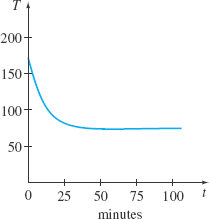
\includegraphics[width=0.37\textwidth]{figs/exercise-5-1-3}
\end{frame}


\begin{frame}{exercise 21 in \S 1.3}

\begin{columns}
\begin{column}{0.75\textwidth}
\scriptsize
\begin{quotation}
\noindent \textbf{21}.  A small single-stage rocket is launched vertically as shown.  Once launched, the rocket consumes its fuel, and so its total mass $m(t)$ varies with time $t>0$.  If it is assumed that the positive direction is upward, air resistance is proportional to the instantaneous velocity $v$ of the rocket, and $R$ is the upward thrust or force, then construct a mathematical model for the velocity $v(t)$ of the rocket.
\end{quotation}

\small
\begin{itemize}
\item hint 1: when the mass is changing with time, Newton's law is
\begin{equation}
F = \frac{d}{dt}\left(mv\right) \tag{17}
\end{equation}
where $F$ is the net force on the body and $mv$ is the momentum
\item hint 2: on page 27 there is a model for air resistance used in equation (14): $F_2 = - k v$
\end{itemize}
\end{column}
\begin{column}{0.3\textwidth}
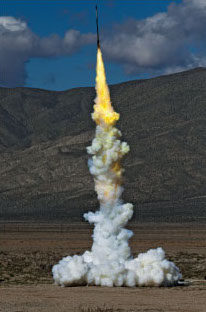
\includegraphics[width=\textwidth]{figs/exercise-21-1-3}
\end{column}
\end{columns}


\end{frame}


\begin{frame}{exercise 21, cont.}

\begin{itemize}
\item collect the forces to get the net force:

$$F = \hspace{70mm}$$
\vspace{10mm}

\item now we can write down the model:

\vspace{30mm}
\end{itemize}
\end{frame}


\begin{frame}{exercise 10 in \S 1.3}

\scriptsize
\begin{quotation}
\noindent \textbf{10}.  Suppose that a large mixing tank initially holds 300 gallons of water in which 50 pounds of salt have been dissolved.  Another brine solution is pumped into the tank at a rate of 3 gallons per minute [gal/min], and when the solution is well-stirred it is then pumped out at a slower rate of 2 gal/min.  If the concentration of the solution entering is 2 pounds per gallon [lb/gal], determine a differential equation for the amount of salt $A(t)$ in the tank at time $t>0$.
\end{quotation}

\small
\begin{itemize}
\item $A(t)$ is amount of salt in pounds [lb]; what is $A(0)$?
\item what is $V(t)$, the total solution volume?
\item write down the differential equation for $\frac{dA}{dt}$:

\vspace{30mm}
\end{itemize}
\end{frame}


\begin{frame}{exercise 10, extended and fully-solved}

\begin{itemize}
\item what is a function $A(t)$ satisfying the ODE IVP?:
    $$\frac{dA}{dt} = 6 - \frac{2}{300+t} A, \quad A(0)=50$$
\item one may verify that

\vspace{-5mm}
    $$A(t) = 2 (300+t) - 550 \left(\frac{300}{300+t}\right)^2$$

\vspace{-2mm}
    \begin{itemize}
    \item get it using methods in \S 2.3
    \end{itemize}

\centerline{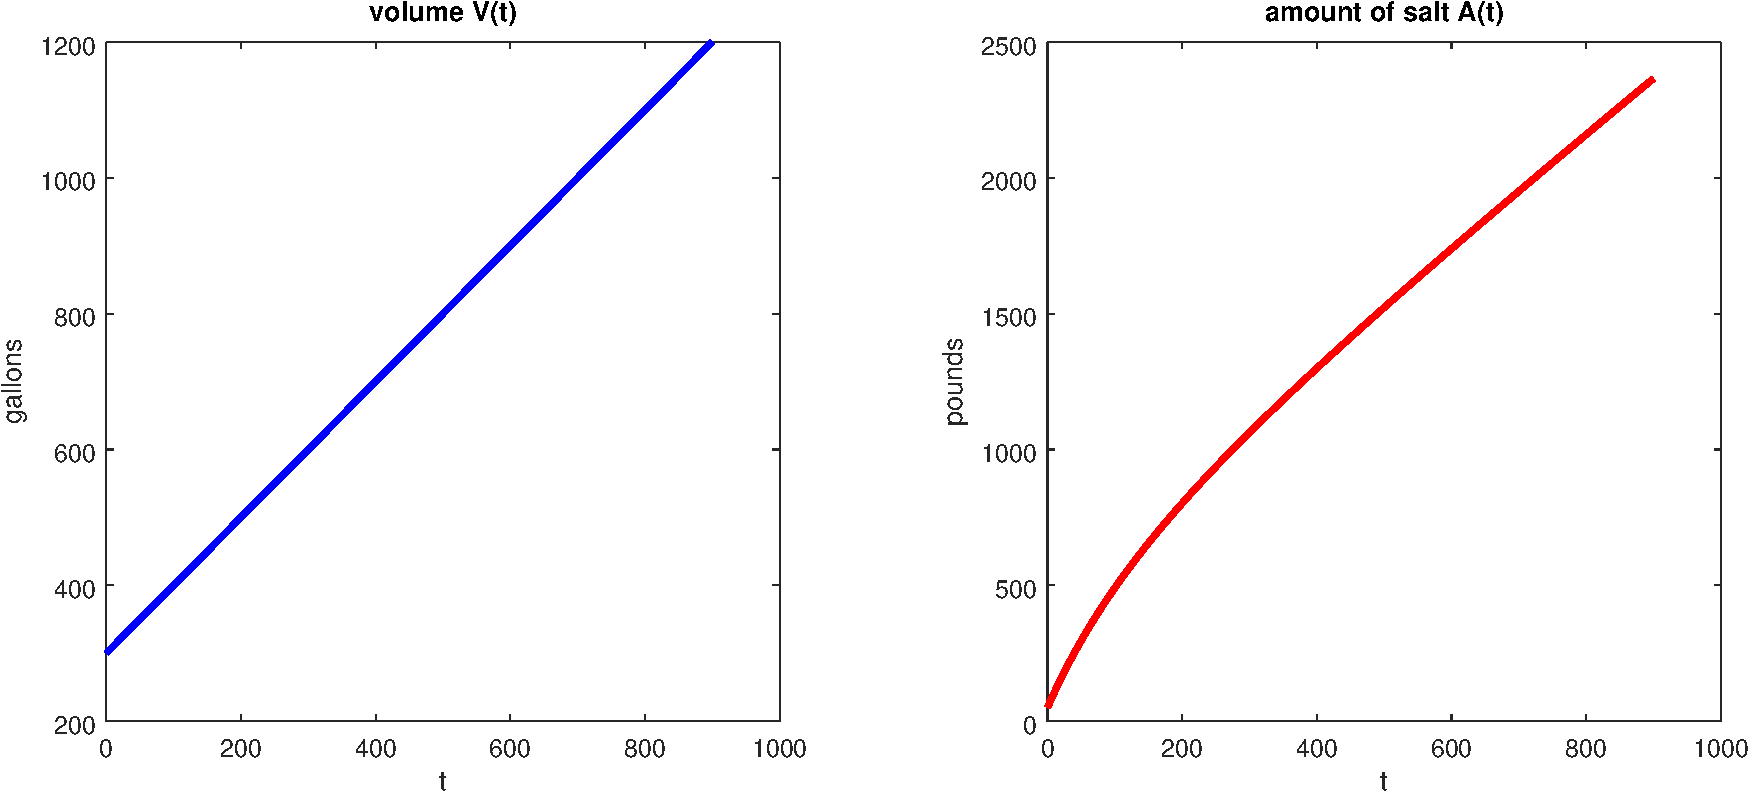
\includegraphics[width=0.8\textwidth]{figs/exercise-10-1-3}}
\end{itemize}
\end{frame}



\begin{frame}{expectations}

to learn this material, just watching this video is \emph{not} enough; also
\begin{itemize}
\item \emph{read} section 1.3 in the textbook
    \begin{itemize}
    \item for instance, actually \emph{read} the ``Mixtures'' example on p.~25 and the ``Falling Bodies and Air Resistance'' example on p.~27
    \end{itemize}
\item \emph{do} the WebAssign exercises for section 1.3
\item see the other ``found online'' videos at the bottom of the week 2 page:

\centerline{\href{https://bueler.github.io/math302/week2.html}{\tt \color{cyan} bueler.github.io/math302/week2.html}}
\end{itemize}
\end{frame}

\end{document}

